\documentclass[11pt]{article}

\usepackage[left=1.25in,top=1.25in,right=1.25in,bottom=1.25in,head=1.25in]{geometry}
\usepackage{amsfonts,amsmath,amssymb,amsthm}
\usepackage{verbatim,float,url}
\usepackage{caption}
\usepackage{graphicx}
\usepackage{framed}
%\usepackage[]{hyperref}
%\usepackage{dsfont,bm}
%\usepackage{harvard}
%\citationmode{abbr}

\def\half{\frac{1}{2}}
\def\th{\mathrm{th}}
\def\sign{\mathrm{sign}}
\def\supp{\mathrm{supp}}
\def\E{\mathrm{E}}
\newcommand{\iid}{\stackrel{\mathrm{i.i.d.}}{\sim}}

\newcommand{\eps}{\varepsilon}
\DeclareMathOperator{\argmin}{argmin}

\def\P{\mathrm{P}}
\def\Var{\mathrm{Var}}
\def\Cov{\mathrm{Cov}}
%\def\R{\mathds{R}} 
\newcommand{\R}{\mathbb{R}}
\def\cA{\mathcal{A}}
\def\cB{\mathcal{B}}
\def\cE{\mathcal{E}}
\def\cF{\mathcal{F}}
\def\cG{\mathcal{G}}
\def\cN{\mathcal{N}}
\def\inv{^{-1}}
\def\hbeta{\hat{\beta}}
\def\trace{\mathrm{trace}}
\global\long\def\ty{\tilde{{ y}}}
\global\long\def\tX{\tilde{{ X}}}
\global\long\def\tx{\tilde{{ x}}}

\title{Data Mining: 36-462/36-662 \\ Homework 1 Solutions}
\author{\bf Due Thursday January 29, 2015 \\
(at the beginning of lecture)}
\date{}

\begin{document}
\maketitle

{\it Append your R code to the end of your homework. In your solutions, you should
just present your R output (e.g., numbers, table, figures) or snippets of R
code as you deem it appropriate. Make sure to present your results (i.e., your
R ouput) in a clear and readable fashion. Careless or confusing presentations 
will be penalized.}

\bigskip
\bigskip
\noindent
{\bf\large Problem 1}
In this problem, we replicate the prediction error plot for regression from
Lecture 3, and then show that ridge regression can be used to reduce the
variance of the estimator, improving the overall MSE.

\bigskip
\noindent
{\bf (a)} Replicate the simulation from class for linear regression, showing
that the prediction error starts at $\sigma^2$ and increases to $2\sigma^2$ as
$p$ approaches $n$.

The simulation has two loops, one over $p$ from 1 to 40, and one over 100
replications for each $p$.

For each $p$ from 1 to 40 and for fixed $n=50$:
\begin{enumerate}
  \item Generate $X\in\R^{n\times p}$ with $x_{ij}\sim N(0,1)$.
  \item Generate $\beta\in\R^p$ with $\beta_1 = 1$ and $\beta_j\sim U[-.2,.2]$
    for $j>1$.
  \item for $k=1\dots,100$, repeat the following, holding $X$ and $\beta$ fixed:
    \begin{enumerate}
      \item Generate $y=X\beta+\eps$, with $\eps_i\iid N(0,1)$
      \item Fit $\hat{\beta}$ by least squares
      \item Generate $y'=X\beta+\eps'$, with $\eps_i'\iid N(0,1)$.  This is a
        new copy of $y$, which we will try to predict with our 
        $\hat{\beta}$ from the previous part.
      \item We will use the values $\hat{y}^k = X\hat{\beta}$ and $y'^k =
        X\beta + \eps'$ to estimate our average prediction error, average squared bias, and
        average variance across the 50 $x_i$ points in part 4.  The superscript
        $k$ is just to keep track of the value from each repetition in our formulas.
    \end{enumerate}
  \item The true values of average prediction error, average squared bias, and
    average variance (lecture 3, slide 19) are all in terms of expected values.
    To approximate these expectations, we use averages over the 100
    repetitions.  Our results are thus averages over both the 100 realizations
    and the 50 data points.  Let $B = 100$ be the number of repetitions, and
    recall that we have $n=50$ points.  Then
    \begin{align*}
      PE &= \frac{1}{n}\sum_{i=1}^n \frac{1}{B} \sum_{k=1}^B \left(y_i'^k -
      \hat{y}_i^k\right)^2\\
      Bias^2 &= \frac{1}{n}\sum_{i=1}^n \left(x_i^T\beta -
      \frac{1}{B}\sum_{k=1}^B \hat{y}_i^k\right)^2\\
      Var &= \frac{1}{n}\sum_{i=1}^n \frac{1}{B}\sum_{k=1}^B \left(\hat{y}_i^k
      - \frac{1}{B}\sum_{k=1}^B \hat{y}_i^k\right)^2
    \end{align*}
    Notice that for the bias and variance terms, you're going to need to sum
    over the 100 realizations at each $x_i$ point before you sum over the 50
    data points.  This is because the mean of your estimator changes as you
    move across the $x_i$.  Luckily, none of these formulas are going to change
    when we switch to ridge regression in part (b) of this problem.

\end{enumerate}

Finally, plot the estimated averaged values (from part 4 above) versus $p$ for
the values $p=1,\dots,40$.  The horizontal axis will be $p$, and the vertical
axis will be each of the averaged values.

You should see the linear increase due to the variance, as we saw in class.

\emph{Note:} Do not be worried if your prediction error starts a little above
1.  The signal in this simulation is a little lower than the simulation I
showed in class, which can shift the starting point.


\bigskip
\noindent

{\bf (b)} What happens if you use ridge regression instead of least squares to
fit $\hat{\beta}$?  Repeat everything from the previous part, but this time
estimate $\hat{\beta}$ using ridge regression instead of least squares.  To do
so, you will have to pick a value $\lambda$.  Try to find a value of $\lambda$
that will give prediction errors which are lower than least squares for the
large values of $p$ (say $p$ from 30 to 40).  When you find a $\lambda$ that
works, include a plot of the prediction, variance, and bias curves for that
$\lambda$. 

For the successful case where the prediction errors are lower than least
squares, how have the bias and the variance of the estimator changed?

\begin{framed}
{\bf\large Solution to Problem 1 (Shashank)}\\
See Figures \ref{fig:problem1linear} and \ref{fig:problem1ridge} for our error
plots and see the Code Appendix on page \pageref{app:code} for our R code. In
general, long code segments should be in an appendix rather than in the middle
of your homework.
%%% BEGIN FIGURE %%%
\begin{center}
  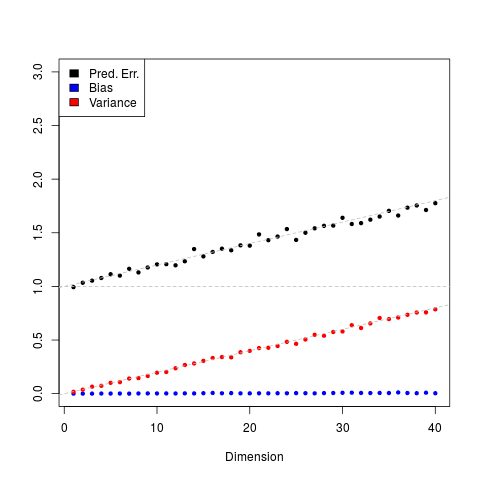
\includegraphics[width=0.68\textwidth]{linear}
\vspace{-5mm}
\captionof{figure}{
Linear regression prediction error, bias, and variance as dimension $p$
varies.}
\label{fig:problem1linear}
  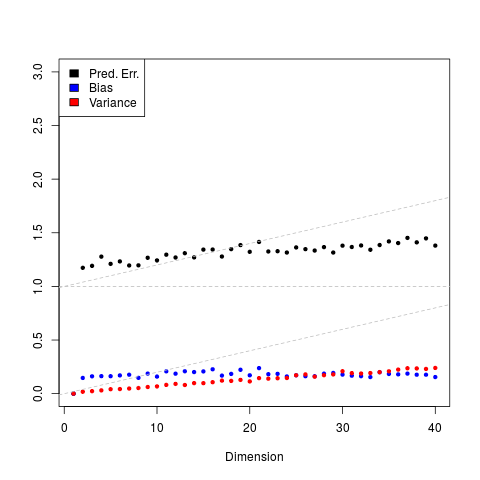
\includegraphics[width=0.68\textwidth]{ridge}
\vspace{-5mm}
\captionof{figure}{
Ridge regression prediction error, bias, and variance as dimension $p$ varies.}
\label{fig:problem1ridge}
\end{center}
%%% END FIGURE %%%

We can see that, in lower dimensions, linear regression outperforms ridge
regression (which has higher bias), but, in higher dimensions, ridge regression
peforms better by controlling the variance of linear regression. When $p = 40$,
\texttt{glmnet} chooses $\lambda \approx 26$, which is what we use here. \\

{\bf Grading:}
\begin{itemize}
\item 10 points for figures (-3 without clear labels)
\item 3 points for discussing $\lambda$
\item 7 points for discussing/comparing error of linear and ridge regression
\item 5 points for reasonable looking code (-2 without basic commenting)
\end{itemize}

{\bf Notes:} Many students chose $\lambda$ too small ($\lambda < 10$). This is
immediately evident from the bias/variance plot because because variance will
continue to dominate bias for all $p$. Typically, to minimize prediction error,
we want to chose $\lambda$ such that the bias and variance are roughly equal.
\end{framed}


\bigskip
\bigskip
\noindent
{\bf\large Problem 2}

\smallskip
\noindent
In class so far, we have been looking at a regime where $n>p$ and $X$ is full
rank.  This problem explores what happens when we depart from those
assumptions.

Consider the usual linear regression setup, with response vector $y \in \R^n$ and
predictor matrix $X \in \R^{n\times p}$. Let $x_1,\ldots x_p$ be the columns
of $X$. Suppose that $\hbeta \in \R^p$ is a minimizer of the least squares 
criterion
\begin{equation*}
\|y-X\beta\|_2^2.
\end{equation*}

\bigskip
\noindent
{\bf (a)} Show that if $v \in \R^p$ is a vector such that $Xv=0$,
then $\hbeta + c\cdot v$ is also a minimizer of the least squares criterion,
for any $c \in \R$.

\bigskip
\noindent
{\bf (b)} If $x_1,\ldots x_p \in \R^n$ are linearly independent, then
what vectors $v \in \R^p$ satisfy $Xv=0$?

\bigskip
\noindent
{\bf (c)} Suppose that $p>n$. Show that there exists a vector $v\not=0$
such that $Xv=0$. Argue, based on part (a), that there are infinitely
many linear regression estimates. Further argue that there is a variable
$i \in \{1,\ldots p\}$ such that the regression coefficient of
variable $i$ can have different signs, depending on which estimate we 
choose. Comment on this. 

\begin{framed}
{\bf\large Solution to Problem 2 (Shashank)}

\begin{enumerate}
\item[{\bf (a)}] {\bf (5 points)}
Since $Xv = 0$, for any $c \in \R$,
\[\|y - X(\hat\beta + c \cdot v)\|_2^2
    = \|y - X\hat\beta + c \cdot Xv\|_2^2
    = \|y - X\hat\beta + c \cdot \vec 0\|_2^2
    = \|y - X\hat\beta\|_2^2.
\]
Hence, $\hat\beta + c \cdot v$ has the same least squares loss as $\hat\beta$
and is also a minimizer.

\item[{\bf (b)}] {\bf (5 points)}
Since $Xv = v_1 \cdot x_1 + \dots + v_p \cdot x_p$ is a linear combination of
the linearly independent set $\{x_1,\dots,x_p\}$ with coefficients
$v_1,\dots,v_p$, $Xv = 0$ implies $v = 0$.

{\bf Note:} This tells us that least squares regression is safe (or at
least well-defined) when our samples span $\R^p$. However, this can only happen
when we have at least $p$ samples.

{\bf Technical Note:} Several students claimed that, because $X$ has linearly
independent columns, it has an inverse $X\inv$. Only square matrices have
proper inverses, with $XX\inv = I = X\inv X$. What is true here is that $X$ has
a \emph{left inverse} $X\inv$ with $X\inv X = I_p$ (but not $XX\inv = I_n$). In
this case, a left inverse is all we need, but not making this distinction can
sometimes lead one to derive false statements.

\item[{\bf (c)}] {\bf (15 points)} Because $Xv$ is a linear combination of $p$
column vectors in $\R^n$, if $p > n$, the columns of $X$ are linearly
dependent. Thus, there exists a particular $v \neq 0$ such that $Xv = 0$.

(Another valid way to phrase this is that the homogeneous linear
system $Xv = 0$ has more variables than equations, and hence has a nonzero
solution $v \neq 0$. You should understand both explanations.)

If we let $\hat\beta$ be a linear regression estimate (i.e., a least-squares
minimizer), part (a) then tells us that, for any of the infinitely many
$c \in \R$, $\hat\beta' = \hat\beta + c \cdot v$, is also a valid linear
regression estimate.

Since $v \neq 0$, some component $v_i \neq 0$, and so, for any $r \in \R$, if
we choose $c = \frac{r - \hat\beta_i}{v_i}$, then
$\hat\beta_i' = \hat\beta_i + c v_i = r$. Thus, $\hat\beta_i'$ could be any
real number, and so we have no way to interpreting the dependence of $y$ on the
covariate $x_i$ in our model.

{\bf Note:} An intuitive way to view this is that each sample imposes a linear
constraint on the $p$-dimensional variable $\beta$ that encodes our model.
Thus, when $p > n$, we have insufficient data to specify the model, suggesting
the need for other constraints (such as a regularization term).
\end{enumerate}
\end{framed}


\bigskip
\bigskip
\noindent
{\bf\large Problem 3}

\smallskip
\noindent
Given a response vector $y\in\R^n$, predictor matrix $X \in \R^{n\times p}$, and tuning
parameter $\lambda \geq 0$, recall the ridge regression estimate
\begin{equation*}
\hbeta^\mathrm{ridge} = 
\argmin_{\beta \in \R^p} \,\|y-X\beta\|_2^2 + \lambda \|\beta\|_2^2.
\end{equation*}

\bigskip
\noindent
{\bf (a)} Show that $\hbeta^\mathrm{ridge}$ is simply the vector of
linear regression coefficients from regressing the response
$\tilde{y}=\left[\begin{array}{c} y \\ 0\end{array}\right] \in \R^{n+p}$
onto the predictor matrix $\tilde{X} = \left[\begin{array}{c} X \\ \sqrt{\lambda}I\end{array}\right]
\in \R^{(n+p)\times p}$, where here $0 \in \R^p$, and $I \in \R^{p\times p}$ is the identity 
matrix.

\bigskip
\noindent
{\bf (b)} Show that the matrix $\tilde{X}$ always has full column-rank, i.e., its columns
are always linearly independent, regardless of the columns of $X$. Hence argue that the
ridge regression estimate is always unique, for any matrix of predictors $X$. 

\bigskip
\noindent
{\bf (c)} Write out an explicit formula for $\hbeta^\mathrm{ridge}$ involving $X,y,\lambda$.
Conclude that for any $a\in\R^p$, the estimate $a^T \hbeta^\mathrm{ridge}$ is a linear function of 
$y$.

\bigskip
\noindent
{\bf (d)} 
Now consider the estimation of $a^T \beta^*$, with $\beta^*$ being the true coefficient vector.
Based on what we've seen in lecture, ridge regression can have a lower MSE than linear regression. 
But on the last homework we proved that the linear regression estimate is the
best linear unbiased estimate (BLUE). Given that it 
is indeed linear (from part (c)), what does this imply about the ridge regression estimate, 
$a^T \hbeta^\mathrm{ridge}$?


\begin{framed}
{\bf\large Solution to Problem 3 (Bryan)}
\begin{enumerate}
\item[{\bf (a)}]
The linear regression objective when regressing $\tilde{{y}}$
onto $\tX$ is: 

\begin{eqnarray*}
\left\| \ty-\tX\beta \right\|_{2}^{2} & = & \left\| \left[\begin{array}{c}
y\\
0
\end{array}\right]-\left[\begin{array}{c}
X\\
\sqrt{\lambda}I
\end{array}\right]\beta \right\|_{2}^{2}\\
 & = & ||y-X\beta||_{2}^{2}+||0-\sqrt{\lambda}I\beta||_{2}^{2}\\
 & = & ||y-X\beta||_{2}^{2}+||\sqrt{\lambda}I\beta||_{2}^{2}\\
 & = & ||y-X\beta||_{2}^{2}+\lambda||\beta||_{2}^{2}
\end{eqnarray*}
which is the objective minimized by ridge regression. Hence the minimizer
of this expression is $\hat{{\beta}}^{\mbox{ridge}}$.

\item[{\bf (b)}] $\tX$ has $p$ linearly independent rows (namely, its last $p$
rows). Since $\tX$ is $(n+p)\times p$, its (row) rank must therefore be $p$.
Recall that row rank equals column rank; therefore, since $\tX$ has $p$
columns, its columns must be linearly independent.


Since $\tX$ has full rank, note that
$\tX^{T}\tX v=0\Rightarrow||\tX^{T}v||_{2}^{2}=0\Rightarrow\tX^{T}v=0$.
Thus $\tX^{T}\tX$ has full rank and the least squares solution $\tilde{\beta}$
from regressing $\tilde{{y}}$ onto $\tX$ is unique, hence
$\hat{{\beta}}^{\mbox{ridge}}$ is unique.

\item[{\bf (c)}] By expanding the least squares solution:
\begin{eqnarray*}
\tilde{\beta} & = & (\tX^{T}\tX)^{-1}\tX^{T}\ty\\
 & = & (\left[\begin{array}{c}
X\\
\sqrt{\lambda}I
\end{array}\right]^{T}\left[\begin{array}{c}
X\\
\sqrt{\lambda}I
\end{array}\right])^{-1}\left[\begin{array}{c}
X\\
\sqrt{\lambda}I
\end{array}\right]^{T}\left[\begin{array}{c}
y\\
0
\end{array}\right]\\
 & = & (X^{T}X+\lambda I)^{-1}X^{T}y
\end{eqnarray*}
It follows that $a^{T}\hat{{\beta}}^{ridge}=a^{T}(X^{T}X+\lambda I)^{-1}X^{T}y$
is a linear function of $y$.

\item[{\bf (d)}] Since the least squares solution has the lowest MSE out of all
unbiased estimators and we showed that ridge regression has lower MSE, it
follows that the ridge regression estimator $a^{T}\hat{{\beta}}^{ridge}$ is
biased.




\end{enumerate}
\end{framed}

\bigskip
\bigskip
\noindent
{\bf\large Problem 4}

\smallskip
\noindent
In this problem you're going to prove the Gauss-Markov theorem.

Recall that the theorem assumes that we observe a vector $y \in \R^n$ of observations
from the model
\begin{equation*}
y = X\beta^* + \epsilon,
\end{equation*}
where $X \in \R^{n\times p}$ is a fixed matrix of predictor variables, $\beta^* \in \R^p$
are the true coefficients, and $\epsilon \in \R^n$ are random errors, with 
\begin{equation*}
\E[\epsilon] = 0, \;\;\; \Cov(\epsilon) = \sigma^2 I.
\end{equation*}
Given a vector $a\in \R^p$, we consider linear unbiased estimates of $a^T \beta^*$. That is,
we consider estimates of the form $c^T y$ such that $\E[c^T y] = a^T \beta^*$. Note that
the regression estimate $a^T \hbeta$ is both linear and unbiased, as 
\begin{equation*}
a^T \hbeta = a^T (X^T X)^{-1} X^T y = \big( X (X^T X)^{-1} a \big)^T y = b^T y,
\end{equation*}
and $\E[a^T \hbeta] = a^T \E[\hbeta] = a^T \beta^*$. As our criterion we use mean squared
error; for any estimate $c^T y$ of $a^T \beta^*$, its mean squared error is
\begin{equation*}
\mathrm{MSE}(c^T y) = \E[(c^T y - a^T \beta^*)^2].
\end{equation*}
The Gauss-Markov theorem states that $a^T \hbeta$ is the best linear unbiased estimate (BLUE) 
of $a^T \beta^*$ in terms of mean squared error, that is,
\begin{equation*}
\mathrm{MSE}(a^T \hbeta) \leq \mathrm{MSE}(c^T y)
\end{equation*}
for any other linear unbiased estimate $c^T y$ of $a^T \beta^*$. You will prove this in
several steps.

\bigskip
\noindent
{\bf (a)} Prove that $\E[y]=X\beta^*$ and $\Cov(y)=\sigma^2 I$.

\bigskip
\noindent
{\bf (b)} Prove that if $\E[c^T y] = a^T \beta^*$ holds for any vector $\beta^* \in \R^p$,
then we must have $X^Tc = a$. 

\bigskip
\noindent
{\bf (c)} Let $c^T y$ be an unbiased estimator of $a^T\beta^*$. Prove that 
$\mathrm{MSE}(c^T y) = \sigma^2 \|c\|_2^2$, and hence
\begin{equation*}
\mathrm{MSE}(c^T y) = \sigma^2 ( \|c^*\|_2^2 + \|c-c^*\|_2^2 )
\geq \sigma^2 \|c^*\|_2^2,
\end{equation*}
with equality if and only if $c=c^*$, where $c^* = P_{\mathrm{col}(X)} \, c$, the
projection of $c$ onto the column space of $X$.

\smallskip
\smallskip
\noindent
(Hint: If $c^T y$ is unbiased, then $\mathrm{MSE}(c^T y) = \Var(c^T y)$.) 

\bigskip
\noindent
{\bf (d)} Prove that $(c^*)^T y = a^T \hbeta$, and conclude that 
$\mathrm{MSE}(a^T \hbeta) \leq \mathrm{MSE}(c^T y)$. 

\smallskip
\smallskip
\noindent
(Hint: Start with $(c^*)^T y = (c^*)^T (\hat{y} + r)$ where $\hat{y}$ is the 
linear regression fit and $r=y-\hat{y}$ is the residual. Then apply the result of 
part (b) to $c^*$.)

\begin{framed}
{\bf\large Solution to Problem 4 (Bryan)}




\begin{enumerate}
\item[{\bf (a)}]
\begin{eqnarray*}
E[y]
    = E[X\beta^{*}+\epsilon]
    = X\beta^{*}+E[\epsilon]
    = X\beta^{*}
\end{eqnarray*}
\begin{eqnarray*}
\mbox{Cov}[y]
    = \mbox{Cov}[X\beta^{*}+\epsilon]
    = \mbox{Cov}[\epsilon]
    = \sigma^{2}I
\end{eqnarray*}
\noindent
\item[{\bf (b)}] We have 
\begin{eqnarray*}
E[c^{T}y] & = & E[c^{T}(X\beta^{*}+\epsilon)]\\
 & = & E[c^{T}X\beta^{*}]+c^{T}E[\epsilon]
   =   c^{T}X\beta^{*}+0
\end{eqnarray*}


Thus the given condition implies $c^{T}X\beta^{*}=a^{T}\beta^{*}$
for all $\beta^{*}$. This is only possible if $c^{T}X=a^{T}$ (for
example, let $\beta^{*}$ be $e_{i}$, the vector with a $1$ in the $i$th coordinate and $0$ elsewhere - then $c^{T}X$ and $a^{T}$ must agree in their $i$th coordinate,
and this holds for each $i$). Tranposing both sides gives $X^{T}c=a$.
\item[{\bf (c)}]
\begin{eqnarray*}
\mbox{MSE}(c^{T}y)
    = \mbox{Var}(c^{T}y)
    = c^{T}\mbox{Var}(y)c
    = c^{T}\sigma^{2}c
    = \sigma^{2}||c||_{2}^{2}
\end{eqnarray*}
Thus by the orthogonality of $c^{*}$ and
$c-c^{*}$,
$\mbox{MSE}(c^{T}y)
    =\sigma^{2}||c||_{2}^{2}
    =\sigma^{2}(||c^{*}||_{2}^{2}+||c-c^{*}||_{2}^{2})
    \ge\sigma^{2}||c^{*}||_{2}^{2}$,
and equality holds iff $||c-c^{*}||_{2}^{2}=0$, i.e. $c=c^{*}$.
\item[{\bf (d)}]
First note that 
\begin{eqnarray*}
E((c^{*})^{T}y) & = & (c^{*})^{T}E(y)\\
 & = & (c^{*})^{T}X\beta^{*}\\
 & =^{(1)} & c{}^{T}X\beta^{*}\\
 & = & E(c^{T}y)\\
 & =^{(2)} & a^{T}\beta^{*}
\end{eqnarray*}
 where $(1)$ holds because $c^{*}$ is the projection of $c$ onto
the column space of $X$, hence $(c^{*})^{T}X=c^{T}X$, and $(2)$
holds because $c^{T}y$ is unbiased. Thus we may apply (b) to show
that $X^{T}c^{*}=a$. Therefore:

\textbf{
\begin{eqnarray*}
(c^{*})^{T}y & = & (c^{*})^{T}(\hat{{y}}+r)\\
 & = & (c^{*})^{T}(X\hat{{\beta}}+r)\\
 & =^{(3)} & (c^{*})^{T}X\hat{{\beta}}\\
 & = & (X^{T}c^{*})^{T}\hat{{\beta}}\\
 & = & a^{T}\hat{{\beta}}
\end{eqnarray*}
}where $(3)$ holds since $c^{*}$ is in the column space of $X$
while $r$ is orthogonal to the column space of $X$.

To show $\mbox{MSE}(a^{T}\hat{{\beta}})\le\mbox{MSE}(c^{T}y)$: from
(c) we have $\mbox{MSE}(c^{T}y)=\sigma^{2}||c||_{2}^{2}\ge\sigma^{2}||c^{*}||_{2}^{2}=\mbox{MSE}(c^{*T}y)$.
It follows that $\mbox{MSE}(a^{T}\hat{{\beta}})=\mbox{MSE}(c^{*T}y)\le\mbox{MSE}(c^{T}y)$. 
\end{enumerate}
\end{framed}

\newpage
\begin{framed}
\label{app:code}
{\bf\large Code Appendix for Problem 1 (Shashank)}
\small
\begin{verbatim}
library(glmnet)
n = 50; p_max = 40; ridge_lambda = 1
reps = 100 # number of trials

## Comment one out
method = "linear" #For linear regression
# method = "ridge" #For ridge regression
bias = numeric(p_max); variance = numeric(p_max); pred_err = numeric(p_max)

for (p in 1:40){
  if (method=='ridge' && p==1){next} # glmnet fails for p = 1, so skip ridge

  X = matrix(rnorm(n*p),ncol=p) # n normal random covariate samples in R^p
  beta = c(1,runif(p-1,-.2,.2)) # beta_1 = 1 and other betas uniformly random
  y_hat = matrix(0,nrow=n,ncol=reps)
  y_prime = matrix(0,nrow=n,ncol=reps)

  for (k in 1:reps){
    y_train = X%*%beta + rnorm(n) # y = X*beta + noise

    if (method=='linear'){
      # lsfit is convenient; important to not include intercept here
      beta_hat = lsfit(X,y_train,intercept=FALSE)$coef
    } else if (method=='ridge') {
      # glmnet returns a sparse vector with an intercept entry, even when the
      # intercept is excluded; this extracts the correct entries as numeric
      beta_hat = as.numeric(coef(
                    glmnet(X,y_train,intercept=FALSE,alpha=0,family='gaussian'),
                s=ridge_lambda)[2:(p+1)])
    }

    y_hat[,k] = X%*%beta_hat # true y
    y_prime[,k] = X%*%beta + rnorm(n) # predicted y
  }
  pred_err[p] = mean((y_prime-y_hat)^2)
  bias[p] = mean((X%*%beta-rowMeans(y_hat))^2)
  variance[p] = mean((y_hat-rowMeans(y_hat))^2)
}
# plot error for each p
plot(1:p_max,pred_err,col='black',ylim=c(0,3),pch=20,xlab="Dimension",ylab="")
points(1:p_max,bias,col='blue',pch=20)
points(1:p_max,variance,col='red',pch=20)
# plot trend lines
abline(a=0,b=1/n,lty=2,col='grey')
abline(a=1,b=1/n,lty=2,col='grey')
abline(h=1,lty=2,col='grey')
legend(legend=c("Pred.Err.","Bias","Variance"),fill=c('black','blue', 'red'))
\end{verbatim}
\end{framed}

\end{document}
